\section{Properties and Shortcuts}
If you have opened the Caesar Perspective, there are some configurations left. Open \markedtext{Window} $\rightarrow$ \markedtext{Customise Perspective}. Check the \markedtext{Caesar} checkbox as shown in figure \ref{fig:propert}.

\begin{figure*}[htbp]
	\centering
		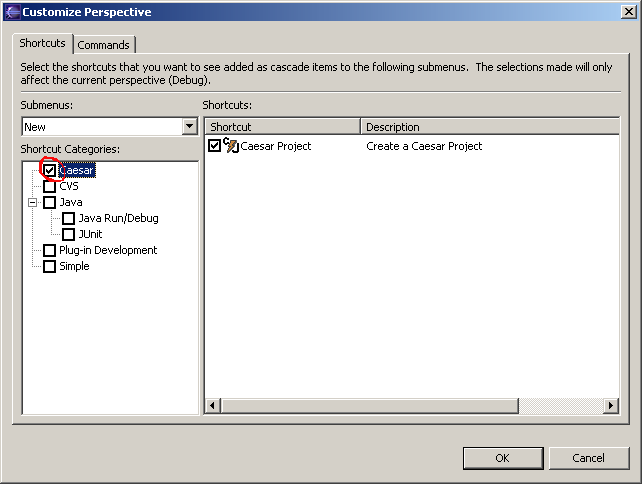
\includegraphics[width=0.60\textwidth]{images/propert.png}
	\caption{Selection the \caesarj ~perspective}
	\label{fig:propert}
\end{figure*}

If this is done, two new Buttons will appear in the toolbar like in figure \ref{fig:toolbar}.

\begin{figure*}[htbp]
	\centering
		
\includegraphics[width=1.0\textwidth]{images/toolbar.png}
	\caption{\caesarj ~toolbar shortcuts}
	\label{fig:toolbar}
\end{figure*}

Figure \ref{fig:properties} shows the \caesarj -Configuration-Wizard, which will be displayed by pressing the \markedtext{P}-Button.

\begin{figure*}[htbp]
	\centering
		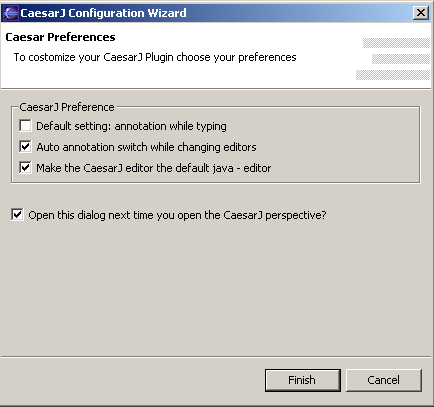
\includegraphics[width=0.60\textwidth]{images/view_properties.png}
	\caption{\caesarj -Configuration-Wizard}
	\label{fig:properties}
\end{figure*}

The \markedtext{A}-Button toggles the "Annotation-While-Typing" option on or off. Even for the Java-Editor.\\
A main feature of the \cjdt ~is the automatic annotation toggling while switching between the \caesarj - and the JAVA-editor. This is a useful feature, because the \cjdt does not support live annotation yet. In this way, \caesarj ~syntax are not marked as wrong expressions.


